\documentclass[11pt,a4paper,twoside]{article}

  \usepackage[T1]{fontenc}
    \usepackage[utf8]{inputenc}
    \usepackage[french]{babel}
    \usepackage{icomma}
	\usepackage{multicol}
    \usepackage{amsmath}
    \usepackage{amsfonts}
    \usepackage{amssymb}
    \usepackage{eurosym}
   	\usepackage{pstricks-add} 
 	\usepackage{pst-tree}
 	\usepackage{color}
 	\usepackage{tabularx}
 	\usepackage{colortbl}
	\usepackage{graphicx}
 	\usepackage[np]{numprint}
 	\usepackage{setspace}
 	\usepackage{listings}
 	\usepackage{hyperref}
    \pagestyle{empty}

\newcommand{\R}{\mathbb{R}}
\newcommand{\N}{\mathbb{N}}
\newcommand{\D}{\mathbb{D}}
\newcommand{\Z}{\mathbb{Z}}
\newcommand{\Q}{\mathbb{Q}}
\newcommand{\C}{\mathbb{C}}

\newcommand{\vect}[1]{\mathchoice%
{\overrightarrow{\displaystyle\mathstrut#1\,\,}}%
{\overrightarrow{\textstyle\mathstrut#1\,\,}}%
{\overrightarrow{\scriptstyle\mathstrut#1\,\,}}%
{\overrightarrow{\scriptscriptstyle\mathstrut#1\,\,}}}
\usepackage{tikzsymbols}
\usepackage{textcomp}
\usepackage{parskip}

\definecolor{mygreen}{rgb}{0,0.6,0}
\definecolor{mygreen}{rgb}{0.43,0.67,0.15}
\definecolor{mygray}{rgb}{0.1,0.1,0.1}
\definecolor{myblue}{rgb}{0.22,0.65,0.85}

\lstset{ 
  upquote=true,
  columns=flexible,
  backgroundcolor=\color{white},
  basicstyle=\large\ttfamily, 
  breakatwhitespace=false,
  breaklines=true,
  captionpos=b,                    % sets the caption-position to bottom
  commentstyle=\color{mygreen},    % comment style
  deletekeywords={...},            % if you want to delete keywords from the given language
  escapeinside={\%*}{*)},          % if you want to add LaTeX within your code
  extendedchars=true,              % lets you use non-ASCII characters; for 8-bits encodings only, does not work with UTF-8
  frame=single,	                   % adds a frame around the code
  keepspaces=true,                 % keeps spaces in text, useful for keeping indentation of code (possibly needs columns=flexible)
  keywordstyle=\color{orange},       % keyword style
  language=Python,                 % the language of the code
  morekeywords={*,...},            % if you want to add more keywords to the set
  numbers=left,                    % where to put the line-numbers; possible values are (none, left, right)
  numbersep=5pt,                   % how far the line-numbers are from the code
  numberstyle=\tiny\color{mygray}, % the style that is used for the line-numbers
  rulecolor=\color{black},         % if not set, the frame-color may be changed on line-breaks within not-black text (e.g. comments (green here))
  showspaces=false,                % show spaces everywhere adding particular underscores; it overrides 'showstringspaces'
  showstringspaces=false,          % underline spaces within strings only
  showtabs=false,                  % show tabs within strings adding particular underscores
  stepnumber=2,                    % the step between two line-numbers. If it's 1, each line will be numbered
  stringstyle=\color{mygreen},     % string literal style
  tabsize=4,	                   % sets default tabsize to 2 spaces
  title=\lstname                   % show the filename of files included with \lstinputlisting; also try caption instead of title
}
\usepackage{geometry}
\geometry{top=1cm, bottom=1cm, left=1cm, right=1cm}

\begin{document}

\begin{center}
\framebox{\textbf{\textsc{TP NSI - Vers le labyrinthe - séance 1 - pygame et bonnes manières}}}
\end{center}
\vskip0.5cm
 
\begin{center}
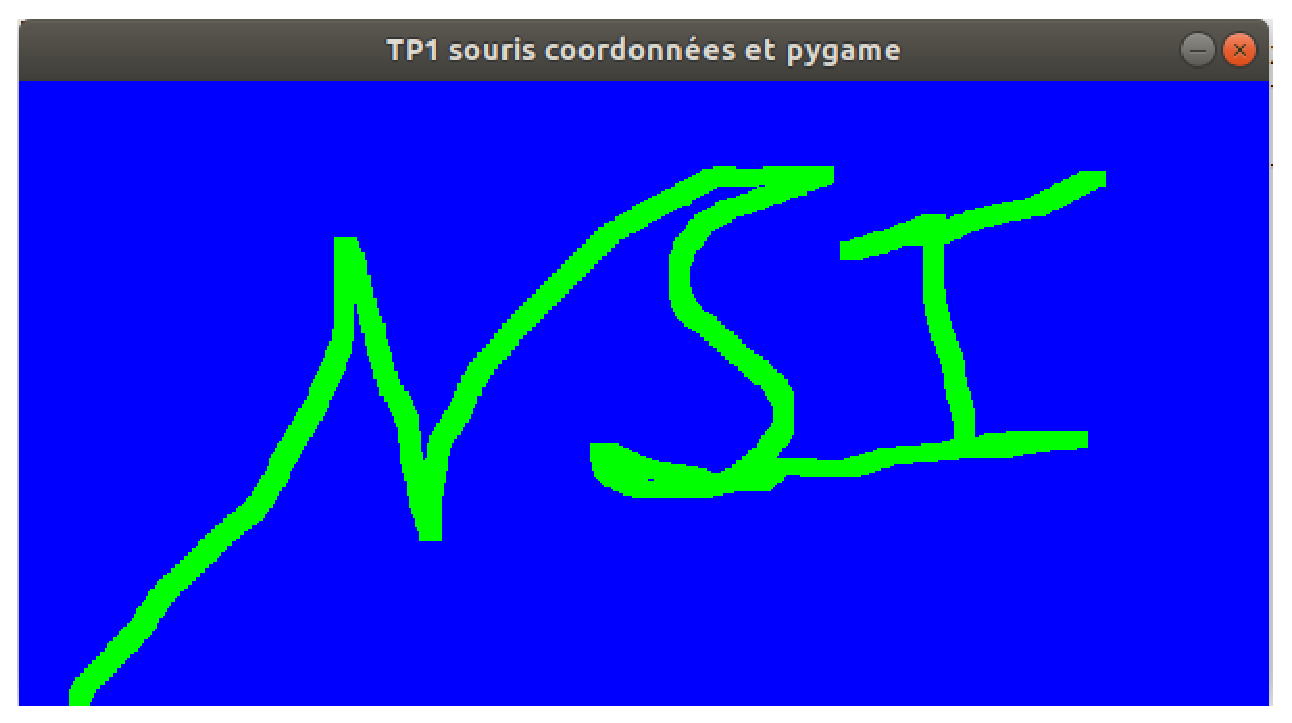
\includegraphics[scale=0.6]{TP1-capture.eps}
\end{center}

\noindent \textbf{Partie 1 : Compréhension du code}\\

Voici le code qui permet de suivre les déplacements de la souris sur la fenêtre crée.\\
Tu le trouveras aussi dans l'espace partagé.\\
Commente chaque ligne du programme en explicitant son but.\\

\begin{center}
\begin{minipage}{16cm}
\lstinputlisting[language=java]{TP1-souris-initial.py}
\end{minipage}
\end{center}
\newpage
\noindent \textbf{Partie 2 : Modification du programme}\\

\noindent 
\begin{enumerate}
\item Modifie le programme pour :\begin{itemize}
\item[•] permettre l'affichage dans la console des coordonnées de la souris lors d'un clic,
\item[•] afficher un cercle centré sur l'endroit du clic.
\end{itemize}
\item Modifie le programme pour :\begin{itemize}
\item[•] ne plus afficher tous les déplacements de la souris mais seulement les 100 derniers déplacements !\\Pour cela il faudra les enregistrer dans une \textsl{liste}.\\
\end{itemize}
\end{enumerate}

\noindent \textbf{Partie 3 : Pour aller plus loin}\\

\noindent Modifie le programme pour changer la couleur du fond en appuyant sur une des flèches du clavier.\\On aura besoin d'introduire trois variables et de modifier le code en ligne 9 ainsi :\\
\begin{center}
\begin{minipage}{16cm}
\begin{lstlisting}[language=Python,firstnumber=9]
rouge,vert,bleu=0,0,255
fenetre.fill((0,0,255))
\end{lstlisting}
\end{minipage}
\end{center}
On modifiera le rouge pour la flèche \og bas \fg{}, le vert pour la flèche \og gauche \fg{} et le bleu pour la flèche \og droite \fg{}.

\end{document}
